\documentclass[journal=jcisd8,manuscript=article]{achemso}
% \linespread{1.5}
\usepackage{amssymb,amsmath,graphics,epsfig}
% \usepackage{amsmath}
\usepackage[font=small,labelfont=bf]{caption}
\usepackage{multirow}
\usepackage{xcolor}
\usepackage{siunitx}
\usepackage{float}
\usepackage{upgreek}
\usepackage{soul}
\setkeys{acs}{super = true}
\setcitestyle{super,open={},close={}}
\def\citenumfont{}

% \usepackage[version=3]{mhchem} 
\usepackage{color}
\newcommand{\eqnref}[1]{Eqn.~\plainref{#1}}
\newcommand{\figref}[1]{Fig.~\plainref{#1}}
\newcommand{\tabref}[1]{Table~\plainref{#1}}

\title{Making Soup: Preparing and Validating Molecular Simulations of the Bacterial Cytoplasm}


\author{Leandro Oliveira Bortot}
\affiliation{Laboratory of Biological Physics, School of Pharmaceutical Sciences of Ribeir{\~a}o Preto, University of S{\~a}o Paulo, Ribeir{\~a}o Preto, Brazil}
\altaffiliation{These authors contributed equally to this work}

\author{Zahedeh Bashardanesh}
\affiliation{Science for Life Laboratory, Department of Cell and Molecular Biology. Uppsala University, SE-751 05 Uppsala, Sweden}
\altaffiliation{These authors contributed equally to this work}

\author{David van der Spoel}
\affiliation{Science for Life Laboratory, Department of Cell and Molecular Biology. Uppsala University, SE-751 05 Uppsala, Sweden}
\email{david.vanderspoel@icm.uu.se}


\begin{document}

\maketitle

\newpage
\begin{abstract}
Biomolecular crowding affects the biophysical and biochemical behavior
of macromolecules when compared to the dilute environment present in
experiments made with isolated proteins. Computational modeling and
simulation are useful tools to study how crowding affects the
structural dynamics and biological properties of macromolecules. As
computational power increased, modeling and simulating large scale
all-atom explicit solvent models of the prokaryote cytoplasm become
possible. In this work, we build an atomistic model of the cytoplasm
of \textit{Escherichia coli} composed of 1.5 million atoms and submit
it to a total of \SI{3}{\micro\second} of molecular dynamics
simulations. The simulation model is consistent with experimental data
about the diffusion coefficient and stability of macromolecules under
crowded conditions. In order to stimulate further work we provide a
Python script and a set of files that enables any researcher to build
their own \textit{E. coli} cytoplasm models to address questions
related to crowding.
\end{abstract}

\newpage
\section*{Introduction}


%Biomolecules move and function in an environment densely packed with high concentrations of macromolecules. The presence of macromolecules leads to steric effect due to excluded volume effect and intermolecular attrative/repulsive forces due to distributed charges on the surface of macromolecules.

The intracellular environment is markedly different from the
\textit{in vitro} model systems from which most of our knowledge about
the biochemical and biophysical behavior of macromolecules has been
derived~\cite{Feig2017a}. The \textit{in vivo} microenvironment is
heterogeneous with high concentrations of many different compounds,
leading to spatial constrains that directly affects biological
activities~\citep{ostrowska2019}. This effect, called macromolecular
crowding, influences the stability of many macromolecules
because the equilibrium is shifted towards a stable native structure
as a result of the entropic component given by the excluded volume
effect~\cite{cheung2005}. At the same time, an effective
destabilization due to the enthalpic component of the Gibbs energy has
been observed, due to replacing interactions with water by weaker
interactions with the
crowders~\cite{Feig2011,miklos2011,Wang2012b}. Additionally, crowding
affects the structure and dynamics of water around proteins, which has
a significant effect on their biological
activities~\cite{Harada2012a,king2013}.

While the structure and dynamics of biomolecules is well characterized
\textit{in vitro}, the understanding of the influences of crowded
environments \textit{in vivo} are still evolving.  Techniques such as
nuclear magnetic resonance~\cite{reckel2007,pielak2008} and
fluorescence spectroscopy~\cite{ignatova2004,xie2008,English2011} are
among the most relevant to the field due to their ability to probe
cells in a non destructive way. Another essential class of methods
come from computational modeling and simulation. By extrapolating the
advances in computational power in the last decades to the future, it
was estimated that the atomistic simulation of an entire
\textit{Escherichia coli} bacterium for \SI{1}{\nano\second} will be
possible in 15 years from now~\cite{vanGunsteren2006a}.
% {\bf THAT WAS 13 YEARS AGO. WHAT IS THE STATE OF THE ART?} {\color{blue} The paper predicts that simulating a whole E. coli bacterium with $10^{11}$ atoms for 1 ns will be possible in 2034, thus the "15 years from now" in our text. That was meant as an introduction to the simulation of big systems. The evolution of computational models to study crowing and the state-of-the-art is discussed in the next paragraph. Maybe we can move this phrase to the beginning of the next paragraph }

As the available computational power increases, models become
increasingly complex and are better representations of reality. The
most simple class of computational models apply Brownian Dynamics
calculations to probe macromolecules immersed in a solution of
crowders that are treated as hard spheres with varying radii to
represent different types of molecules~\cite{Ando2010}. These models
usually use an implicit representation of the
solvent~\cite{Mcguffee2010}. More recently, all-atom explicit solvent
molecular dynamics simulations have been employed on crowded systems
composed of several copies of one or a few
macromolecules~\cite{Wang2017c}. However, these models do not reflect
the true heterogeneity of biologically relevant crowded environments
such as the cytoplasm. This was addressed by the development of a
detailed model for the cytoplasm of the bacterium \textit{Mycoplasma
  genitalium} containing 103 million atoms~\cite{Feig2015}. This
model, as well as a smaller version with 13 million atoms, was
submitted to molecular dynamics simulations~\cite{Yu2016a}. Due to the
size of these systems, the simulation times were very short,
\SI{20}{\nano\second} for the complete model and
\SI{140}{\nano\second} for a smaller version, precluding an accurate
characterization of dynamical effects that can take place in such a
large scale. It was noted already some years ago that even
{microsecond} simulations may be too short to probe the dynamics of
large complexes like viruses~\cite{Larsson2012a} since dynamics is
slower in larger systems in general.

In this work, we report an all-atom model of part of the cytoplasm of
\textit{Escherichia coli} was built to reflect the real biological
system, in particular as regards a realistic composition of this
``soup''. We discuss the difficulties that arise when building such a
system and provide a set of Python scripts and files that anyone can
use to build its own crowded systems with custom parameters and
compounds. Additionally, we performed long molecular dynamics
simulations of our cytoplasm model, reaching \SI{3}{\micro\second} of
total simulation time. To the best of our knowledge, this work is the first to explore the
structural dynamics of an all-atom explicit solvent cytoplasm model 
with microsecond scale molecular dynamics simulations. 


\section*{Materials and Methods}

\subsection{Initial structures}
The protein and tRNA structures were downloaded from the Protein Data
Bank (PDB)~\cite{pdb}. Proteins structures that were either from {\em
  E. coli} or its closest homologues (Table
\ref{tbl:protein_fraction}) were selected for this work. In case of
PDB IDs 1U22 (MetE protein) and 2EIP (Ppa protein), we used a
loop-closure modeling tool based on the Random Coordinate Descent
(RCD) method~\cite{Chys2013} to model missing residues. The four
metabolites were parametrized using the General Amber Force Field
(GAFF)~\cite{Wang2004a} and Antechamber~\cite{Wang2005b} using RESP
charges~\cite{Bayly1993a} that were derived from electron density
calculated at the HF/6-31G* theory level with Gaussian16.  Properties
of compounds modeled using the GAFF have been evaluated in a number of
papers~\cite{Caleman2012a,sprenger2015general,Fischer2015a,JZhang2015a,Spoel2018a}
and strengths and weaknesses are well understood. Here, GAFF is used
for compatibility with the Amber99SB-ws force field~\cite{Best2014a}
used for the biomolecules.
 
 
 
\subsection{General simulation setup}
The cytoplasm model was built at a 30\% biomolecular mass fraction and
a physiological salt concentration of 0.15 mol/L KCl. Dropplets containing each component of the model surronded by water and counter-ions were inserted in an empty box in random positions and orientations. Since the volume of this box was initially bigger than what was strictly necessary to accomodate all components, the system was allowed to shrink in a short simulation. Details about how the simulation box was built and optimized are in the results section. All
simulations were performed with the GROMACS 2018
package~\cite{Abraham2015a,Pronk2013a} using the Amber99SB-ws force
field~\cite{Best2014a}, a modified version of the Amber99SB force
field, in combination with the TIP4P/2005 water
model~\cite{Abascal2005b} and improved K$^+$ parameters~\cite{Dang1995a} to avoid the formation of KCl crystals that is observed when using the default parameters of the Amber99SB force field~\cite{Auffinger2007a}. All interactions were calculated explicitly
inside a 1 nm radius and long range electrostatic interactions were
treated using the particle mesh Ewald
algorithm~\cite{Essmann1995a}. Corrections due to long range effects
of dispersion interactions were made to both energy and
pressure~\cite{Allen1987a}. All chemical bonds were constrained at
their equilibrium length using the parallel LINCS
algorithm~\cite{Hess1997a,Hess2008b} allowing an integration time step
of 2 fs. Temperature was kept at 310 K by the v-rescale
thermostat~\cite{Bussi2007a} with a coupling constant of 0.5
ps. Pressure was kept at 1 bar using the Berendsen
barostat~\cite{Berendsen1984a} with the coupling constant of 10.0 ps
during thermalization steps and by the Parrinello-Rahman
barostat~\cite{Parrinello1981a} with the same coupling constant during
production steps.

All systems were initially submitted to energy minimization with the
steepest descent algorithm until convergence to machine (single)
precision. For the cytoplasm model, a short shrinking step of 500 ps
was performed in order to allow the box volume to adjust to its
optimal value. For all systems, initial velocities were sampled from a
Maxwell-Boltzmann distribution at 310 K and we ran a 1 ns NVT
thermalization step followed by 10 ns of NPT equilibration. Production
runs for the dilute systems, in which each crowder is simulated alone
in a water box, had a- length of 200 ns. The cytoplasm model was run
for 1 \SI{}{\micro\second}. All systems were simulated in three
replicas. While the replicas for the diluted systems were generated by
different initial velocities, each replica of the cytoplasm model is a
completely different box in which the components of the model are in
different positions and orientations.

\subsection{Analyses}
For statistics, the average and standard error of the three trajectories are reported. For values that
are specific to each chain, we used the average over the individual
chains in each trajectory of the replicas. Additionally, since there
is more than one copy of some crowders in the cytoplasm models,
average values and standard errors are calculated considering each copy of each replica. As in the dilute system, separate chains of each copy
of the crowders were considered as independent samples when running
analyses that focus on one single chain. The first half of all
simulations was discarded as equilibration time and analyses used only
the second half.

Analyses were done using GROMACS tools after removing artifacts
generated by periodic boundary conditions from the trajectories. A
Mean Square Displacement (MSD) analysis was performed to calculate the
translational diffusion coefficient, which were extracted by a linear
fit to MSD by averaging blocks with a length of $10\, ns$ for dilute systems and $100\, ns$ 
for cytoplasm system~\cite{Allen1987a}. In principle, diffusion
coefficient needs to be corrected for finite size
effects~\cite{Yeh2004,Abraham2018}. Due to relatively large simulation boxes
this correction is negligible. 
% {\bf NOT FOR PROTEINS THAT DIFFUSE
  % SLOWLY!}. {\color{blue} The correcion in Yeh2004 is derived for cubic simulation boxes, in our single molecule simulations we have non-cubic boxes, one needs to derive the correction from Eq 11 in Yeh2004. My Mathematica skills are rusty now, could you do that? If you think it's absolutely necessary} 
Root Mean Square Deviation (RMSD) and Root Mean Square
Fluctuation (RMSF) calculations considered the C$\upalpha$ atoms only for analysis in each trajectory.
% {\bf ARE YOU SURE? THE DEFAULT IS TO TAKE THE AVERAGE STRUCTURE. OR DO  YOU MEAN THE STRUCTURE FOR FITTING?} {\color{blue} I checked and indeed we used the average structure calculated with the second half of the trajectories. I removed "the reference frame for RMSF was the midpoint of the time interval" from the text. The information about the second half of the trajectory is in the previous paragraph, which is about statistics}. 
The chain interface area of a given oligomer in a given
frame was calculated as the difference between the solvent exposed
surface area (SASA) of the oligomer in that frame and the sum of the
SASAs of each of its chains independently in that same frame. Other
analyses, such as box volume and Radial Distribution Function (RDF),
followed standard procedures.

\section*{Results}

\subsection{Cytoplasm model}
In this section we describe the rationale behind the composition of
our model, which consists of five fractions: protein, RNA, metabolites, water
and ions. It should be noted that we did not add lipids and DNA to our
model because we consider only elements that are free to diffuse
through the cytosol. We gathered data from several sources in order to
build a computational model that is representative of the cytoplasm of
{\em Escheria coli}~\cite{Dong1996,Bennett2009,Link1997,Mcguffee2010}.

\subsubsection{Protein fraction}
Eight different proteins were selected that together account for 50\%
of the non-ribosomal proteins in the cytoplasm of {\em Escherichia
  coli} \cite{Link1997}. The two most abundant proteins, TufA and
MetE, account for about 20\% and 12\% of the total protein abundance
in {\em E. coli}, respectively, while the other six proteins
contribute with less than 5\% each (Table~\ref{tbl:protein_fraction}).
The least abundant protein was present with 1 copy and the amount of
each of the other proteins was taken to be an integer number of
oligomers. This was done because the original oligomeric state for
each protein was kept as reported in their crystallographic structure
(Table~\ref{tbl:protein_fraction}).

\begin{table}[H]
\centering
\caption{Protein, PDB ID, number N of proteins in the simulation. 
Fraction of the total abundance of non-ribosomal proteins in the cytosol of {\em
    E. coli} K12 and oligomeric state of each protein that was
  selected to compose our cytoplasm model.}
\label{tbl:protein_fraction}
\begin{tabular}{ccccc}
\hline
Protein & PDB & N & Fraction [\%] & State\\
\hline
Elongation factor TU (TufA) & 1DG1~\cite{Abel1996}       & 6 & 19.7 &  dimer \\
Cobalamin-independent methionine synthase (MetE) & 1U22~\cite{Ferrer2004}     & 7 & 11.6 &  monomer \\
Isocitrate dehydrogenase (IcdA) & 1P8F~\cite{Mesecar2000}    & 2 & 4.7  &  dimer \\
Alkyl hydroperoxide reductase subunit C (AhpC) & 1YEP~\cite{Parsonage2005}  & 1 & 4.1  &  decamer \\
Cold-shock protein (CspC) & 1MJC~\cite{Schindelin1994} & 3 & 4.0  &  monomer \\
Pyrophosphatase (Ppa)  & 2EIP~\cite{Kankare1996}    & 1 & 2.9  &  hexamer \\
Glyceraldehyde 3-phosphate dehydrogenase A (GapA) & 1S7C~\cite{ShinXXX}        & 1 & 2.1  &  tetramer \\
Enolase (Eno)  & 1E9I~\cite{Kuhnel2001}     & 1 & 1.9  &  dimer \\
\hline
Total &                           & 48& 51.1 & \\
\hline
\end{tabular}
\end{table}


\subsubsection{RNA fraction}
Transporter RNAs (tRNAs) account for 74\% of the dry weight of
non-ribosomal RNAs~\cite{phillips2012}. Thus, we chose to model the
RNA presence in the cytoplasm with tRNA molecules. Specifically, 
 the tRNA(Phe) molecule as a representative of tRNAs due to
the availability of a recent crystal
structure (4YCO~\cite{Byrne2015}). The protein and RNA content of the total
dry weight of \textit{E.coli} is 55\% and 2.9\%,
respectively~\cite{phillips2012}. That is, the total RNA weight
corresponds to 5\% of the total protein weight. This protein/RNA
weight ratio was used to calculate the correct number of tRNA(Phe)
molecules that were added to the cytoplasm model
\tabref{tbl:soup_components}.

\subsubsection{Metabolites fraction}
The most abundant molecules of each metabolite class was used to 
represent the class, i.e. Glutamate (GLT) for amino acids, ATP for
nucleotides, Fructose-2,6-Biphosphate (FBP) for central carbon
intermediates and Glutathione (GSH) redox
cofactors~\cite{Bennett2009}. The total number of molecules was
calculated considering data showing that the number of metabolite
molecules in the cytoplasm of \textit{E. coli} is $\approx$ 43 times
higher than the number of proteins~\cite{Bennett2009}. The copy number
for each molecule was calculated from the ratios between their
experimentally observed concentration in {\em
  E. coli}~\cite{Bennett2009}.

\subsubsection{Water fraction}
The number of water molecules was calculated according to the desired
biomolecular concentration, which is a parameter of the cytoplasm
model. Macromolecular concentration ranges from 300 to 400 g/L in biological systems
such as \textit{E. coli} cytoplasm~\cite{Zimmerman1991}, the highest concentration corresponds to volume occupation as high as 40\%~\cite{Ellis2003a}. In our case, we
choose a biomolecular concentration of 30\%, that is, the number of
molecules necessary to reach a ratio of total biomolecular mass to
water mass of 30\% was inserted into the cytoplasm model.

\subsubsection{Inorganic ions fraction}
Finally, Mg\textsuperscript{2+} was used as counter-ions for tRNA and
ATP. K$^{+}$ and Cl$^{-}$ were added to neutralize the charges of the
simulation box and to reach the ionic strength of 0.150 mol/L by
substitution of randomly selected water molecules.



\begin{table}
\centering
\begin{tabular}{lcc}
\hline
Class & Name & Number\\
\hline
RNA & tRNA$^{\text{Phe}}$ & 5\\
\hline
Metabolite & GLT & 1436\\
  & ATP & 144\\
  & FBP & 225\\
  & GSH & 255\\
\hline
Solvent & Water & 306221\\
\hline
Inorganic Ion & K$^{+}$ & 4602\\
  & Mg$^{2+}$ & 400\\
  & Cl$^{-}$ & 1320\\
\hline
\end{tabular}
\caption{Number of copies for non-protein components of the cytoplasm model built at the biomolecular fraction of 30\%.}
\label{tbl:soup_components}
\end{table}



\subsection{Building the simulation box}
All components can be put in the same simulation box by inserting each
of them in random orientations in a cubic volume of side $L$ that is
initially empty. However, that is not a trivial process. We need to
use a box size that is big enough to allow the random insertions to
succeed without structural overlapping and without creating artificial
interactions between the elements by placing them too close from each
other. On the other hand, as the box gets bigger, it gets harder to
equilibrate the system because the empty space between the components
will induce the barostat to reduce the box volume quickly during the
simulation.

We devised an iterative process that solves both problems
simultaneously. We start with a box size $L$ that is too small to
allow all components to fit in the box by random insertion. In our
case, we start with $L = 30$ nm. Then, we allow 100 insertion trials
for each element. If all trials fail for any of them, we start the
whole process again with an empty cubic box that is larger by a step
size $dL$ of 1 nm. We repeat this process until all insertions
succeed. In our case, all insertions succeeded after increasing $L$ to
35 nm. Additionally, instead of adding only the protein, tRNA or
metabolite molecules in the empty box in each trial, we actually add a
droplet of water and counter ions in which the molecule of interest is
embedded. Such droplets are taken from molecular dynamics simulations
in which each component was previously equilibrated. The benefits of
using such droplets are threefold: \textit{i.} it acts as natural
protecting layer that prevents artificial contacts between the
components that could be created due to the random
insertions. \textit{ii.} it is a natural way to place water molecules
and counter-ions in the simulation box around each
component. \textit{iii.} the components are already pre-equilibrated,
which will help us to perform the equilibration of the whole cytoplasm
model.

In order to do this, the droplets around each component are also
constructed iteratively. The number of water molecules that we must
place in the simulation box is known from the total biomolecular mass
of the system and the desired biomolecular fraction, which is a
parameter of the model. However, we don't know the thickness of the
water layer around each component, $l$, that accounts for such amount
of water molecules \textit{a priori}. Since $l$ depends on a series of
factors such as the shape, size and abundance of each element, we
define it iteratively. We start by taking a droplet of thickness $l$ =
3 \r{A} around all elements and counting the number of water molecules
that we would add to the box with such droplets. If it is smaller than
the number we need, $l$ is increased by $dl$ = 1 \r{A}. If it is
larger, we reduce the droplet thickness by $dl$, reduce $dl$ by 10
times and then increase $l$ with the new smaller $dl$. We can carry
this process until a user-defined precision cutoff, here 5\%, for the
number of waters in the system is satisfied.


After all droplets are successfully inserted in a simulation box by
the iterative process described above, we proceed to add ions to
neutralize the net charge of the system and to reach the desired ionic
strength. Then, we perform energy minimization and a short simulation
 of 500ps in which all molecules of the box are free to move. In
this step the box shrinks to its optimum size. In our case, the
simulation box shrank from the initial box size of 35 nm to 22.9 nm,
which corresponds to a volume change from 42875 nm\textsuperscript{3}
to 12009 nm\textsuperscript{3}. From this point, the system is ready
to be submitted to the default simulation steps such as thermalization
and production run (please check the materials section for details
about the parameters used).

\begin{figure}[H]
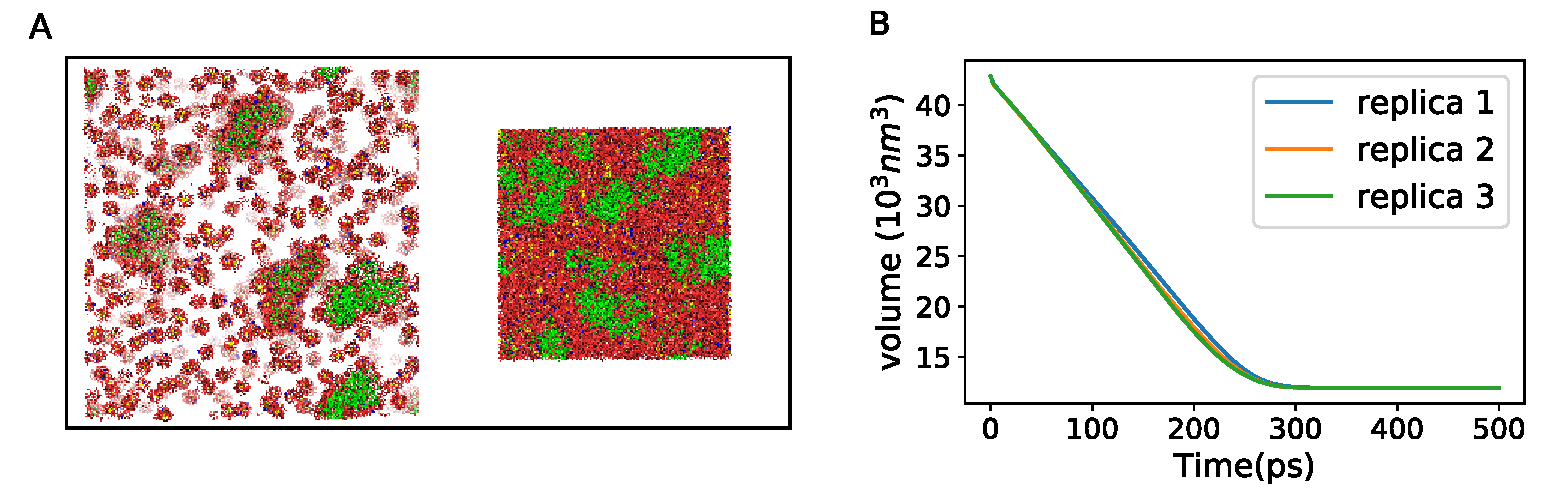
\includegraphics[scale=0.5]{shrinking.pdf} 
\caption{A) The initial simulation box with $L=35.0$ nm and the box
  after the shrinking step, $L=22.9$ nm. B) The evolution of the
  volume of the simulation box during the shrinking simulations. Each
  replica is shown in different colors. }
\end{figure}

\subsection{Effects of macromolecular crowding}

In order to investigate the effects of crowding in the
\textit{E. coli} cytoplasm model on the structural integrity and
dynamics of its elements, we constructed three completely independent
cytoplasm models that have different orientations for each of its
elements. We submitted these systems, each composed of more than 1.5
million atoms, to molecular dynamics simulations of
\SI{1}{\micro\second}. We also performed \SI{200}{\nano\second}
molecular dynamics simulations for each isolated element (proteins and
tRNA) in order to represent the non-crowded, i.e. dilute environment
(please check the materials section for details about the parameters).



\subsubsection{Translational diffusion}

Under crowded conditions, molecules are confined to a smaller
effective volume by the other components of the environment.  The
extent of this effect is evident when we compare the translational
diffusion constant of each component in the cytoplasm model,
$D_{cyto}$, and in a dilute system, $D_{dil}$
(Fig.~\ref{fig:translational_diffusion}A). The ratio of these
quantities is independent of the protein size and is always close to
0.13 (Fig.~\ref{fig:translational_diffusion}B). However, the effect of
crowding on the translational diffusion of tRNA is two times
larger. Its $D_{cyto}/D_{dil}$ is 0.07, indicating that its movement
is especially constrained in the crowded environment
(Fig.~\ref{fig:translational_diffusion}B, crowder with 25 kDa),
however, see below.

\begin{figure}[H]
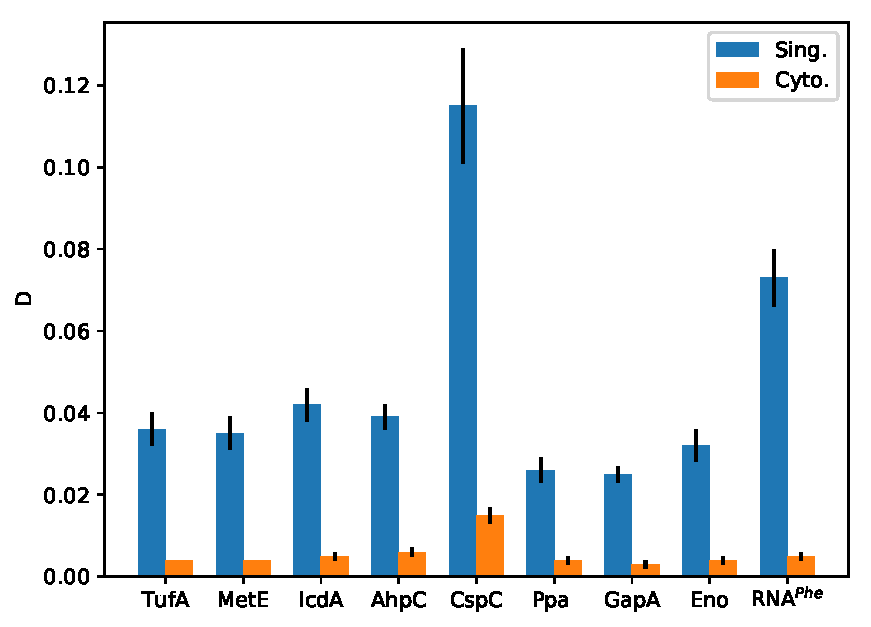
\includegraphics[scale=0.5]{msd.pdf}
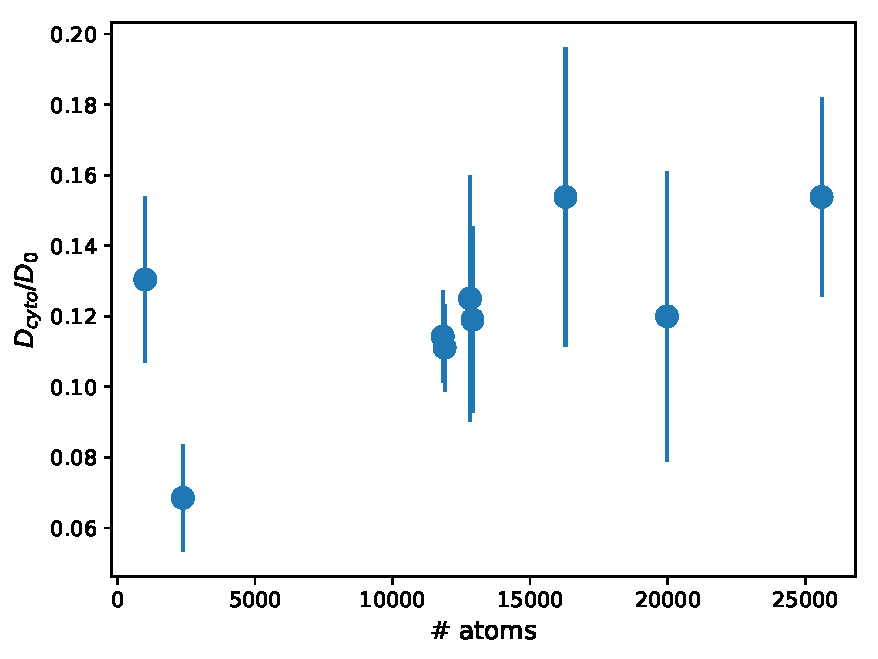
\includegraphics[scale=0.5]{diff_cyto_over_singles.pdf}
\caption{A) Diffusion coefficient of crowders from simulations under
  diluted conditions (blue bars) and cytoplasm simulations (orange
  bars). B) The ratio between diffusion coefficient obtained from
  simulations under both conditions. The crowders are sorted according
  to their sizes on the x-axis.}
\label{fig:translational_diffusion}
\end{figure}

\subsubsection{tRNA is aggregating}
After inspecting the trajectories of the cytoplasm models, we found
that the reason why the translational diffusion constant for tRNA was
reduced to a greater extent than for the other components of the
cytoplasm model is that it was forming aggregates with Mg$^{2+}$, ATP
and FBP (Fig.~\ref{fig:tRNA_aggregation}). Thus, we will omit the tRNA
molecules in the analyses about the structural integrity of the
crowders. In the next sections we will further investigate such
aggregation and we will show a way to prevent it.

\begin{figure}[H]
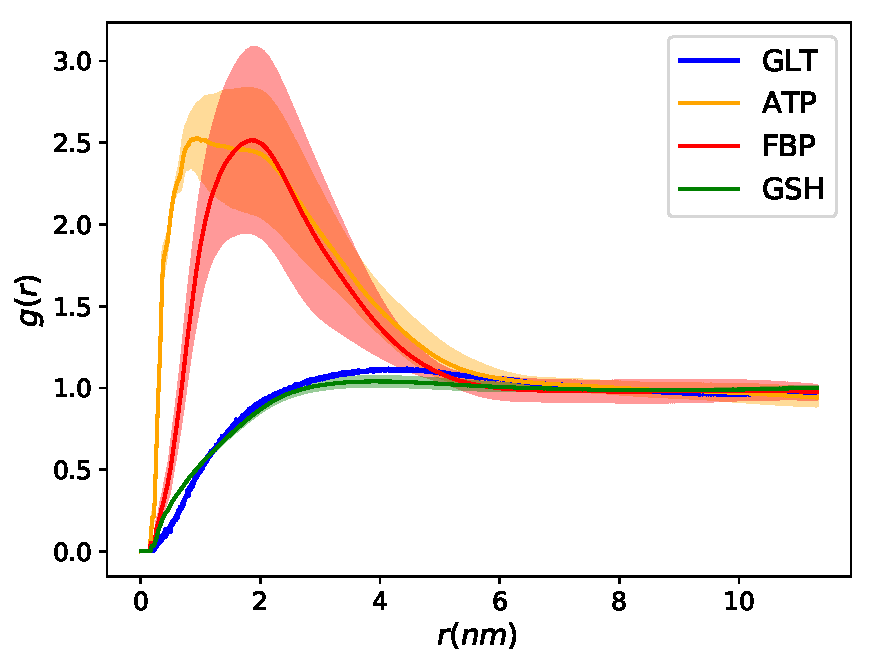
\includegraphics[scale=0.5]{rdf_RNA_metabolites.pdf}
\caption{Radial distribution function showing the probability of
  finding metabolites or Magnesium cations around tRNA molecules in
  the cytoplasm model. Note that ATP and FBP are much more
  concentrated around tRNA than the other metabolites, GSH and GLT.}
\label{fig:tRNA_aggregation}
\end{figure}


\subsubsection{Structural integrity}
The structure of the individual chains of the crowders that were used
in our cytoplasm model were not affected to a great extent by the
crowded environment. The values of their root mean square deviation considering only
their C$\upalpha$ in the cytoplasm model increased by less than 11\% when compared to the dilute condition, except for
TufA, MetE and IcdA, which have RMSD values 105, 25 and 33\% higher in
the crowded environment than in the dilute condition (Fig.~\ref{fig:structural_integrity_chain}A). 
Visual inspection of the final frames of the simulations of these crowders in the cytoplasm model and in dilute condition revealed that, for TufA, the conformational differences are on the $\upbeta$-hairpin around residues 40-62. This region is called Switch I and is known to be flexible and to display conformational changes due to interactions with the ribosome or other partners~\cite{Abel1996}. For MetE, there are differences in the conformation of the loop around residues 450-460 and in the C-terminal $\upalpha$-helices. This loop is known to be flexible and was not modeled in the crystallographic structure due to such flexibility~\cite{Ferrer2004}. For IcdA, the differences are located at the N-terminal coil formed by residues 1-8.

  %{\bf IS THERE A KNOWN PHYSIOLOGICAL REASON FOR THAT?. IS  MetE A MULTIDOMAIN PROTEIN WHERE DOMAINS MOVE WITH RESPECT TO EACH  OTHER?} {\color{blue} The differences of TufA and MetE can be expected from some experimental data, but for IcdA it is just partial unfolding of a short N-terminal coil region.}

The effect of crowded environment on the structural integrity of
oligomers can be evaluated by their chain interface area as well. This
quantity is the solvent accessible surface area that is removed from
access to the solvent by oligomerization. Our results show that
oligomers are not significantly disturbed in the cytoplasm model when
compared to the diluted condition. Similarly to what can be seem by
the RMSD values, which reflect the structural integrity of individual
chains, the oligomers that undergo the most change is TufA
(Fig.~\ref{fig:structural_integrity_chain}B).

\begin{figure}[H]
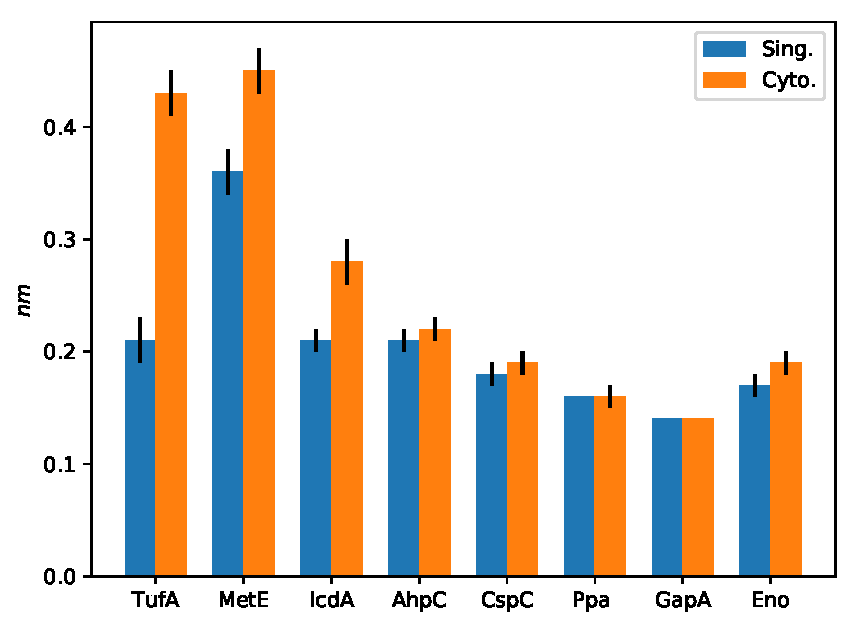
\includegraphics[scale=0.5]{rmsd.pdf}
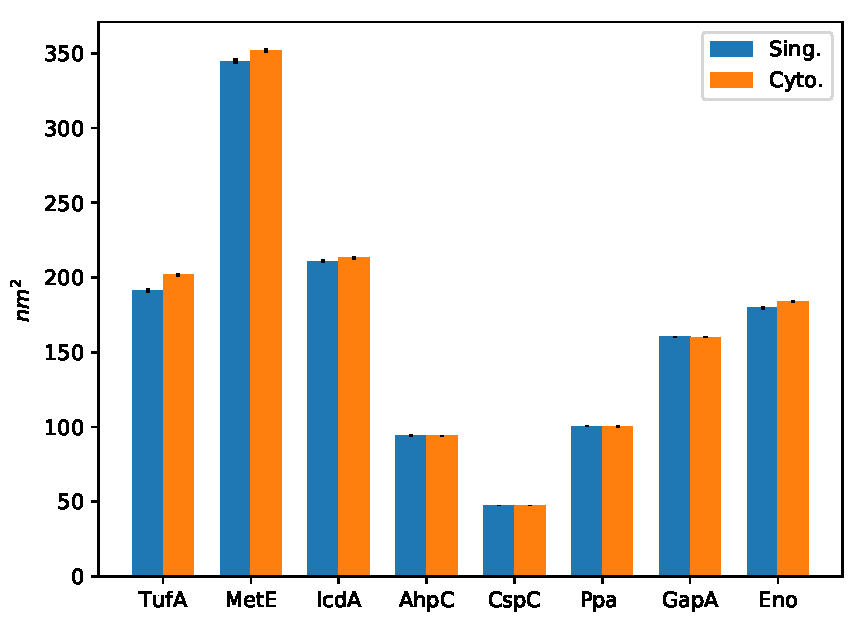
\includegraphics[scale=0.5]{sasa.pdf}
\caption{A) RMSD for all protein crowders from simulations under
  diluted conditions (blue bars) and in the cytoplasm model (orange
  bars). This value reflects the structural integrity of individual
  chains of each crowder. B) Chain interface area for oligomers under
  diluted conditions (blue bars) and in the cytoplasm model (orange
  bars). This value reflects the structural integrity of oligomers of
  the crowders.}
\label{fig:structural_integrity_chain}
\end{figure}



\subsubsection{Structural dynamics}
% {\bf THIS PARAGRAPH REPEATS AND CONTRADICTS ITSELF. IS FLEXIBILITY
%   AFFECTED OR NOT? FROM THE GRAPH I WOULD SAY THE THE FIVE PROTEINS
%   NOTED BELOW ARE MUCH MORE FLEXIBLE, NOT SLIGHTLY. ONE WAY OF
%   QUANTIFYING THIS IS TO COMPUTE THE AVERAGE OF THE MEAN SQUARE
%   FLUCTUATION OVER THE WHOLE PROTEIN, THAT IS BEFORE TAKING SQUARE
%   ROOTS OF COURSE AND PLOTTING THAT IN A BAR GRAPH.} {\color{blue} Overall, flexibility (meaning the values of RMSF for each residue) is affected in some cases, but the flexibility profile (meaning the overall shape of the RMSF plot) is not. Maybe that was the source of the apparent contradiction. I changed the text to clarify that. I also removed words such as "slightly" and "small" from the text.}
  
Root mean square fluctuation (RMSF) calculations show that, overall, the shape of residue-wise flexibility profile of the proteins is not affected by crowding, which is in agreement with our results showing that their structural integrity does not change significantly in the cytoplasm model in most cases (Fig.~\ref{fig:rmsf}). Accordingly, we can see significant changes in the shape of the flexibility profile for regions that undergo conformational changes, such as the Switch I $\upbeta$-hairpin of TufA around residues 40-62 and the flexible loop of MetE around residues 450-460 (Fig.~\ref{fig:rmsf}).

In most cases (TufA, MetE, AhpC, CspC and Ppa), the residue-wise RMSF values are higher in the cytoplasm model than under diluted conditions, which indicates that proteins are more flexible in the cytoplasm model (Fig.~\ref{fig:rmsf}). This is in agreement with computational and experimental data showing that nonspecific interactions with crowders can lead to destabilization of
proteins~\cite{Feig2011, miklos2011, Wang2012b}.

\begin{figure}[H]
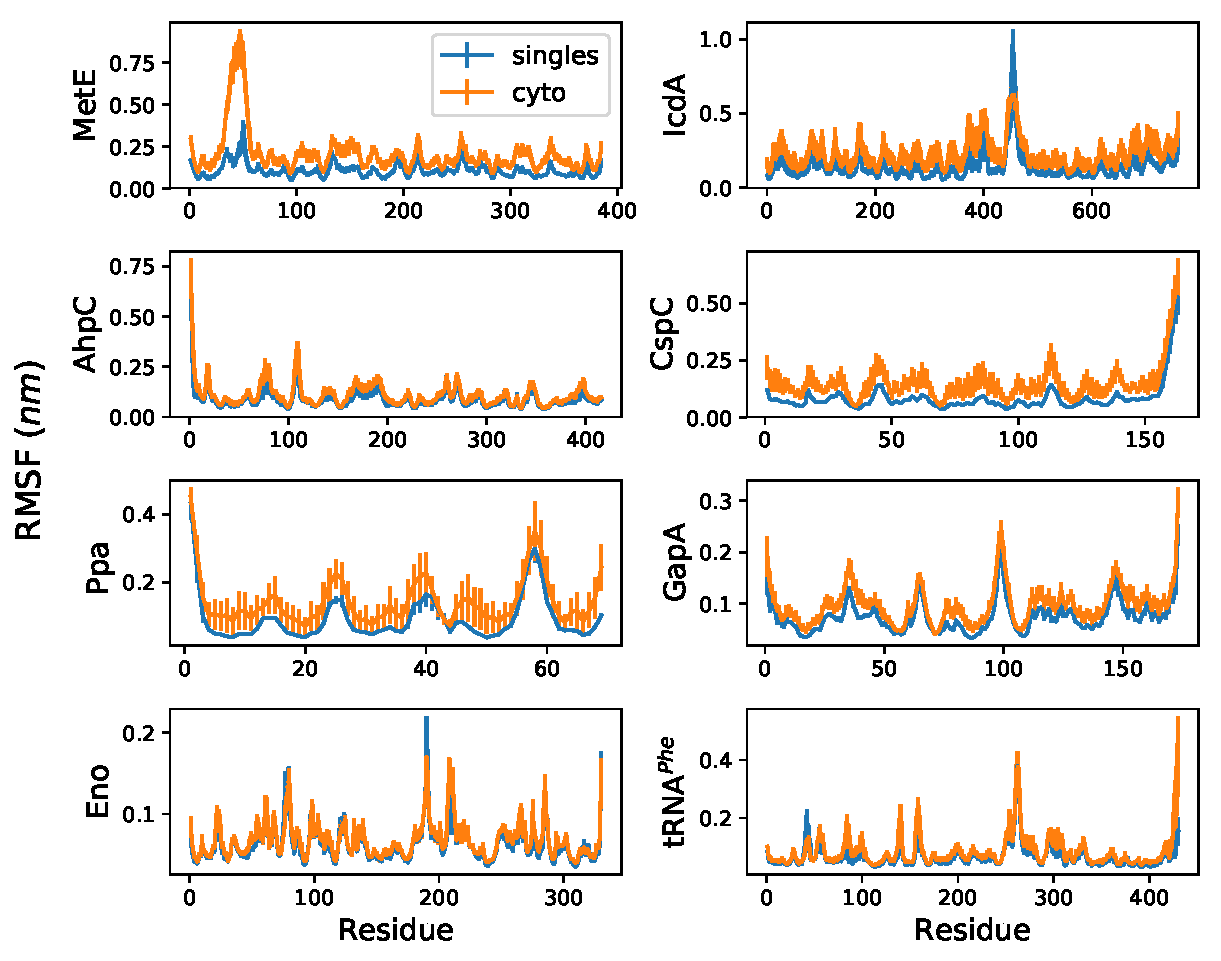
\includegraphics[scale=0.5]{rmsf.pdf}
\caption{Root mean squared fluctuations (RMSF) from simulations under
  diluted conditions (blue bars) and in the cytoplasm model (orange
  bars). The x-axis shows the residues for each chain of proteins.}
\label{fig:rmsf}
\end{figure}






\subsubsection{Aggregation can be avoided by protonating the metabolites}

The initial detection of aggregation in the cytoplasm model was due to
the outlier behavior of the translational diffusion constant of tRNA
when compared to the other crowders. However, tRNA was not the cause of this
phenomenon. Instead, it was triggered by the exaggerated interactions
between the phosphate-containing metabolites, ATP and FBP, with
Mg$^{2+}$ (Fig.~\ref{fig:avoiding_aggregation}A). tRNA gets involved
in the aggregates because Mg$^{2+}$ is present in the box only as
counter-ion for ATP and tRNA, and so tRNA is one of the few
``sources'' of Mg$^{2+}$ in the whole system. We looked for ways of
avoid aggregation by using simulations of small systems composed of
these metabolites in high concentration, Mg$^{2+}$ and water (please
check the methods section for details).

We found that completely protonating the phosphate groups of ATP and
FBP is enough to prevent their aggregation with Mg$^{2+}$. While RDFs
show that ATP$^{-3}$ and FBP$^{-4}$ aggregate around Mg$^{2+}$
(Fig.~\ref{fig:avoiding_aggregation}A), this is not observed for
ATPH\textsubscript{3} and
FBPH\textsubscript{4}(Fig.~\ref{fig:avoiding_aggregation}B-C).  
% {\bf
%   WERE ANY INTERMEDIATE PROTONATIONS TESTED? E.G. FBPH2(2-) AND ATPH(2-)?
%   COMPLETELY PROTONATING IS UNPHYSICAL AS WELL AT THE PH STUDIED. FOR E COLI THE PH SHOULDBE ROUGHLY 7.4 https://en.wikipedia.org/wiki/Cytosol} {\color{blue}I didn't try intermediate protonations, but this can be done in about 1 week if necessary. The physiological states of FBP and ATP at pH 7.4 would be the ones we used originally in the soup. So, in this sense, any protonated state could be called unphysical or unrealistic. We discuss the tradeoffs of using this unphysical protonated state in the discussion section}

\begin{figure}[H]
\hspace*{-2cm}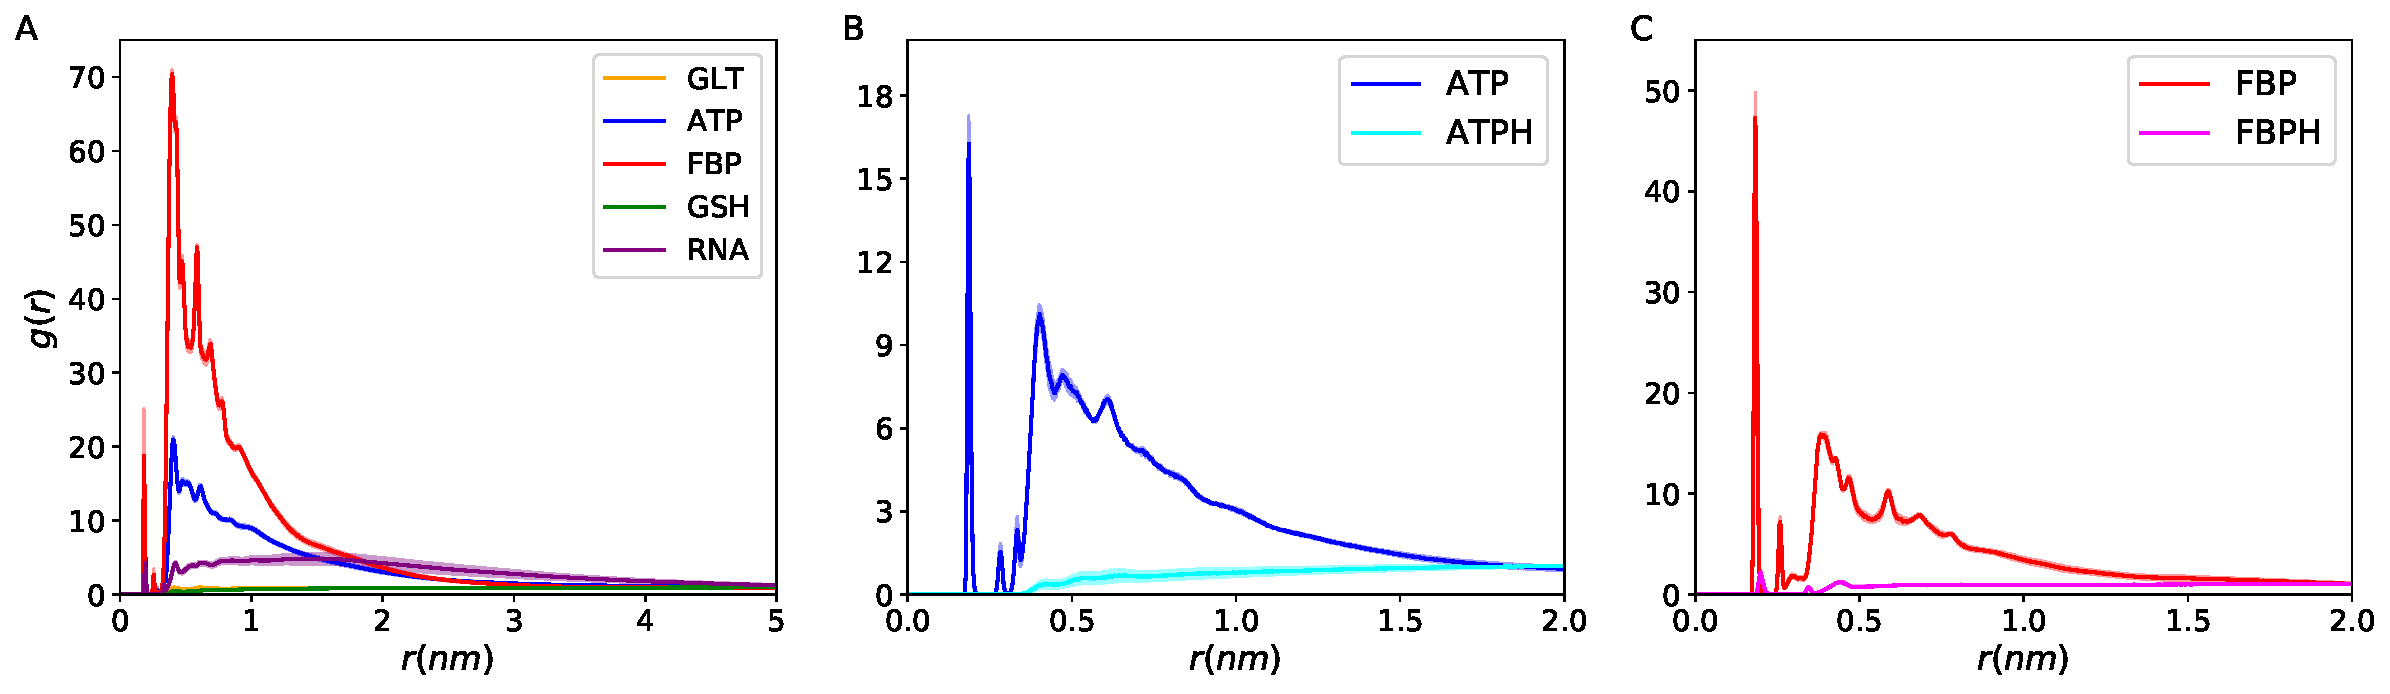
\includegraphics[scale=0.5]{rdf_mg.pdf}
\caption{RDFs centered around Mg$^{2+}$ showing the probability of
  finding A) metabolites in the cytoplasm model, B) ATP$^{-3}$ and
  ATPH\textsubscript{3} or C) FBP$^{-4}$ and FBPH\textsubscript{4} in
  small independent systems (please see the methods section for
  details).}
\label{fig:avoiding_aggregation}
\end{figure}


 

\section*{Discussion}\label{sec:dissc}
The main difference between the behavior of the macromolecules that
compose our model in the crowded system and in the dilute condition is
their translational diffusion coefficient, which drops by around
85\% for the proteins and 93\% for the tRNA
(Fig.~\ref{fig:translational_diffusion}A). The slope of the line
generated by fitting a linear regression model to values of
$D_{cyto}/D_{dil}$ is close to zero (slope $= 0.00028$), showing that
the drop in diffusion coefficient is independent of the size of the
macromolecules. We found that the aggregation of ATP$^{-3}$ and
FBP$^{-4}$ around Mg$^{2+}$, which was used as counter-ion for tRNA,
leads to an exaggerated confinement of the tRNA molecules.  Therefore,
tRNA is considered as an outlier in the duffusion calculations. In
fact, the slope of the linear regression line fitted to
$D_{cyto}/D_{dil}$ is reduced by by 50\% and gets even closer to zero
(slope $= 0.00014$) after removing the diffusion coefficient of tRNA
from the data. These data are in agreement with experimental results
showing that the translational diffusion coefficient of Green
Fluorescent Protein (GFP) in {\em E. coli}, as measured by
fluorescence recovery after photo-bleaching (FRAP), decreased 90\%
when compared to {\em in vitro}
measurements~\cite{Elowitz1999,Konopka2006}.

% {\bf IT MAY BE NECESSARY TO DISCUSS RMSF HERE AS WELL} {\color{blue} This first paragraph is focused on validation of the cytoplasm model by comparison with experimental results, which are available for the translational diffusion coefficient. We don't have specific experimental data that we can compare our RMSF data to. Should we add RMSF here anyway? There is a discussion about our RMSF results some paragraphs ahead in which we compare our data with general trends that were experimentally observed.}

It has been demonstrated that the force fields that are most widely
used to perform molecular dynamics simulations of macromolecules yield
different results for highly concentrated amino acid
solutions~\cite{andrews2013}. Moreover, it has been reported that
simulations of highly concentrated environment leads to aggregation
when additive force fields are used~\cite{Petrov2014a,Abriata2015a,
  Nawrocki2017a} and several approaches have been proposed to
eliminate this
problem~\cite{Best2014a,Piana2015a,Bashardanesh2018b}. Apart from
protein-water interactions, the London-dispersion coefficients in the
force fields have been investigated as well but their effect on
protein-protein interactions seems to be
minor~\cite{Mohebifar2017a,Walters2018a,Bashardanesh2018b}.  A
comparison at the amino acid level shows that none of the Amber family
of force fields combined with different water model can simultaneously
produce high accuracy Gibbs energies of hydration and amino acid side
chain mobility~\cite{HZhang2018a}. Of the different combinations
tested in that work the Amber99sb-ws~\cite{Best2014a} in conjunction
with the TIP4P/2005 water model~\cite{Abascal2005b} was deemed the
best compromise~\cite{HZhang2018a}. Nevertheless, in a related paper
we find signs that the increased interaction between protein and water
may be slightly too strong as it leads to partial unfolding of a
protein~\cite{Bashardanesh2019a}.

Previous
all-atom simulations of large scale cytoplasm models used parameters from the CHARMM family of
force fields~\cite{Yu2016a}. In this work we use a modified version of
the AMBER FF99SB force field in which the solvent-solute interactions
are 10\% stronger~\cite{Best2014a} to study crowding effects on a
cytoplasm model. This force field was chosen because it was corrected
to reproduce experimental data when there are many proteins in the
same simulation box. This force field or similarly adjusted one were also used for studying crowding effect on simpler systems of high concentration of proteins~\cite{Nawrocki2017a,nawrocki2019,Bashardanesh2019a}. All-atom explicit solvent molecular dynamics simulations have been reported for large-scale cytoplasm models of
\textit{Mycoplasma genitalium} composed of 103- and 12-million atoms
that were simulated for 20 and 60 \SI{}{\nano\second},
respectively~\cite{Yu2016a}. The cytoplasm model described in this
work has 1.5 million atoms and was simulated for the total of
\SI{3}{\micro\second}, an unprecedented time scale to study crowding effects on a heterogeneous cytoplasm model in atomic detail.  

Three crowders (TufA, MetE and IcdA) displayed greater deviation from
their crystallographic structure in the cytoplasm model when compared
to the dilute condition, indicating that there was some degree of
local unfolding
(Fig.~\ref{fig:structural_integrity_chain}A). Interestingly, oligomers
were marginally less stable in the cytoplasm model than in the dilute condition.
(Fig.~\ref{fig:structural_integrity_chain}B) and the flexibility
profiles calculated considering the C$\upalpha$ for each chain of the
elements of our cytoplasm model show that, in the crowded condition,
most of the proteins (TufA, MetE, AhpC, CspC and Ppa) are more flexible than in the dilute condition (Fig.~\ref{fig:rmsf}). This
is in agreement with previous simulations~\cite{Feig2011} and
experiment~\cite{miklos2011,Wang2012b} showing that crowders can
destabilize the native structure of proteins due to the numerous
unspecific short-lived interactions that are formed between them in a
crowded environment. A study of protein properties at increasing
concentration showed only few interactions between proteins of the
same type~\cite{Bashardanesh2019a}. The only specific interaction we antecipate between the components of our cytoplasm model is between TufA and tRNA (PDB ID 1TTT is an example of such complex)~\cite{nissen1995crystal}. The TufA-tRNA complex is not present in our simulation boxes even after \SI{1}{\micro\second} of simulation starting from random orientations.

% {\color{blue} We highlight that there are no specific interactions described between the proteins that were used in our cytoplasm model.} {\bf do we expect specific interactions between the proteins in our cyto model? In that case write that with references, otherwise write that there are no known specific interactions between these proteins.} {\color{blue} The only specific interaction we antecipate between the components of the soup is that TufA interacts with tRNA (PDB ID 1TTT is an example of such complex). However, since we are ignoring tRNA in our analyses, I did't mention it. PS: I checked and the TufA-tRNA complex is not present in the last frames of our replicas.}


Magnesium cations were added to our cytoplasm model as counter-ions
for tRNA and ATP. However, as the simulation progressed, FBP and ATP
aggregated around Mg$^{2+}$ and, by consequence, around tRNA
% {\bf,
%   effectively removing the counter ions from the RNA. IS THAT
%   CORRECT?} {\color{blue} No, Figure \ref{fig:tRNA_aggregation} shows that Mg$^{2+}$ is still concentrated around tRNA in the soup }. 
  After identifying this problem, we used simulations of
small systems containing only the metabolites, Mg$^{2+}$ and water to
test different strategies to prevent aggregation in future studies
using long simulations of cytoplasm models. We found that protonating
the phosphate-containing metabolites is enough to reach this goal
(Fig.~\ref{fig:avoiding_aggregation}). Even though ATPH$_3$ and
FBPH$_4$ are not the biologically relevant forms of these molecules in
physiological pH, using their protonated forms may be an acceptable
compromise between parametrization complexity and practical
results. The biggest impact of this approach is on long range
interactions of these metabolites with other molecules due to the
neutralization of their net charge. However, molecules in a crowded
environment are restrained to smaller volumes and shorter inter
molecular distances, which mitigates the effect of charge
neutralization. It has been suggested that charged species should
employ scaled charges in order to be compatible with the empirical
water models~\cite{Leontyev2009a,Leontyev2011a}. Due to the high local
density of negative charges in FBP and ATP this might indeed be an
alternative solution, barring use of polarizable
models~\cite{Ponder2010a,Lopes2013a,Ghahremanpour2018b,Walz2018a}.


To the best of our knowledge, there is only one published study on large scale cytoplasm models that
included metabolites with all-atom explicit solvent molecular
dynamics~\cite{Yu2016a}. Although these authors did not report
aggregation, they mention that the translational diffusion of highly
charged phosphate-containing metabolites is ``much slower'' than
expected in their system. They attributed this observation to
non-specific interactions between such metabolites and proteins. Maybe
aggregation also contributed to their slower diffusion but it was not
evident during their \SI{140}{\nano\second} simulation.

%\section*{Conclusions}\label{sec:concl}

In this work we built an all-atom explicit solvent cytoplasm model
composed of proteins, tRNA, metabolites, inorganic ions and water for a total
of 1.5 million atoms (Table \ref{tbl:soup_components}). The identity
and amount of each component of the model was chosen based on
experimental data about the composition of the cytoplasm of
\textit{E. coli}~\cite{Dong1996,Bennett2009,Link1997,Mcguffee2010}.

We submitted this model to a total of \SI{3}{\micro\second} of
molecular dynamics simulations using a modified AMBER FF99SB force
field that was tuned to reproduce experimental data of systems
composed of several macromolecules~\cite{Best2014a}. The model was
validated by comparing to experimental data about the reduction of the
translational diffusion coefficient of proteins in the cytoplasm of
\textit{E. coli} when compared to the dilute condition (Figure
\ref{fig:translational_diffusion})~\cite{Elowitz1999,Konopka2006}. Additionally,
our data is in agreement with recent simulation work and experimental data
that show that the unspecific interactions between macromolecules in a
crowded environment can destabilize
them~\cite{Feig2011,miklos2011,Wang2012b}. Specifically, we can see
that, despite the overall stability of our cytoplasm model even in the
\SI{}{\micro\second} timescale, the proteins are slightly less stable
in the cytoplasm model than in dilute condition (Figures
\ref{fig:structural_integrity_chain} and \ref{fig:rmsf}).


%Phosphate-containing metabolites FBP and ATP aggregated around Mg$^{2+}$ that were used as counter-ions for ATP and tRNA (Figure \ref{fig:tRNA_aggregation}). We used independent simulations of small systems to evaluate different strategies to prevent such aggregation and found that this can be done by completely protonating these molecules (Figure \ref{fig:avoiding_aggregation}). In the specific case of ATP and FBP modeled with GAFF and simulated in boxes where they are highly concentrated in the presence of Mg$^{2+}$, we advise that they should be completely protonated even though that is not their physiological protonation state. In principle it is possible to develop new parameters for phosphate and Mg that doesn't lead to aggregation. However this is outside of the scope of this study.

As part of this work we are providing Python scripts with a set of
structure and topology files that any researcher can use to build
their own \textit{E. coli} cytoplasm models. Such models can be used
to investigate research questions about the effects of
crowding on specific systems of interest or about crowding
itself. With the files we are providing it is possible, for example,
to add a probe protein to investigate the effect of crowding on it, to
add new macromolecular or small crowders, evaluate the effects of
 temperatures and change the biomolecular concentration to
increase or decrease the intensity of the crowding effect. We
highlight that, since we have already validated it, researchers can
take advantage from building their own cytoplasm models even if they
do not have access to the infrastructure that is necessary to perform
long molecular dynamics simulations. With modest computatioanal power
it is possible, for example, to build many independent snapshots of
the cytoplasm of \textit{E. coli}. All files are publicly available at
http://github.com/dspoel/soup.

 
\bibliography{library}

% \begin{addendum}
%  \item  
%  \item[Competing Interests] 
%  \item[Correspondence]  
% \end{addendum}
 
\end{document}


